\documentclass[10pt]{beamer}

\usetheme{CambridgeUS}
\usepackage[english, russian]{babel}
\usepackage[utf8]{inputenc}
\usepackage{caption}
\usepackage{etoolbox}
\usepackage{multicol}
\usepackage{listings}
\usepackage{color}

\definecolor{mygreen}{rgb}{0,0.6,0}
\lstset{
  basicstyle=\ttfamily\footnotesize,        % the size of the fonts that are used for the code
  breaklines=true,                 % automatic line breaking only at whitespace
  captionpos=b,                    % sets the caption-position to bottom
  commentstyle=\color{mygreen},    % comment style
  keywordstyle=\color{blue},       % keyword style
  stringstyle=\color{red},     % string literal style
  showstringspaces=false,
  morekeywords={include, printf},
  texcl=true     %<---- added
}

\title[\href{https://goo.gl/NRgp8K}{https://goo.gl/NRgp8K} (Term 3)]{ODR, компиляция и линковка}
\author[Гусев Илья]{Гусев Илья}
\institute[МФТИ] 
{Московский физико-технический институт\\*}
\date{Москва, 2017}
\subject{Computer Science}

\begin{document}

\begin{frame}
  \titlepage
\end{frame}

\begin{frame}{Содержание}
\tableofcontents
\end{frame}

\section{Исходный код}
\subsection{Объявления и определения}

\begin{frame}[fragile]{Declaration vs definition}{Declaration}
\begin{enumerate}
\item A declaration may introduce one or more names into a translation unit or redeclare names
introduced by previous declarations. If so, the declaration specifies the interpretation and attributes of these
names.
\item Проще говоря, объявление(declaration) - всего лишь имя. Влиять она может лишь на компиляцию, шаблоны и, например, аргументы функций.
\item {Примеры объявлений:
    \begin{lstlisting}[language=C++]
    extern int a; // declares a
    extern const int c; // declares c
    int f(int); // declares f
    struct S; // declares S
    typedef int Int; // declares Int
    extern X anotherX; // declares anotherX
    using N::d; // declares d
    \end{lstlisting}
}
\end{enumerate}
\end{frame}

\begin{frame}[fragile]{Declaration vs definition}{Declaration}
A declaration is a definition unless:
\begin{enumerate}
\begin{multicols}{2}
\item contains the extern specifier or a linkage-specification
\item doesn't contain an initializer,
\item doesn't contain function body,
\item a function without specifying the function’s body, 
\item a static data member in a class definition, 
\item a class name declaration, 
\item an opaque-enum-declaration, 
\item a template-parameter, 
\vfill\eject
\item a parameter-declaration in a function declarator that is not the declarator of a function-definition
\item a typedef declaration,
\item an alias-declaration, 
\item a using-declaration, 
\item a static\_assert-declaration, 
\item an attribute declaration,
\item an empty-declaration, 
\item a using-directive.
\end{multicols}
\end{enumerate}
\end{frame}


\begin{frame}[fragile]{Declaration vs definition}{Declaration}
Примеры определений:
    \begin{lstlisting}[language=C++]
    int a; // defines a
    extern const int c = 1; // defines c
    int f(int x) { return x+a; } // defines f and defines x
    struct S { int a; int b; }; // defines S, S::a, and S::b
    struct X { // defines X
        int x; // defines non-static data member x
        static int y; // declares static data member y
        X(): x(0) { } // defines a constructor of X
    };
    int X::y = 1; // defines X::y
    enum { up, down }; // defines up and down
    namespace N { int d; } // defines N and N::d
    namespace N1 = N; // defines N1
    X anX; // defines anX
    \end{lstlisting}
\end{frame}

\begin{frame}[fragile]{Declaration vs definition}{Больше примеров}
\begin{lstlisting}[language=C++]
// This is the definition of a uninitialized global variable
int x_global_uninit;
// This is the definition of a initialized global variable
int x_global_init = 1;
// This is the definition of a uninitialized global variable, 
// albeit one that can only be accessed by name in this C file 
static int y_global_uninit;
// This is the definition of a initialized global variable, 
// albeit one that can only be accessed by name in this C file
static int y_global_init = 2;
// This is a declaration of a global variable that exists somewhere
// else in the program
extern int z_global;
// This is a declaration of a function that exists somewhere else 
// in the program (you can add "extern" beforehand if you like, 
// but it's not needed)
int fn_a(int x, int y);
\end{lstlisting}
\end{frame}

\begin{frame}[fragile]{Declaration vs definition}{Больше примеров}
\begin{lstlisting}[language=C++]
// This is a definition of a function, but because it is marked as
// static, it can only be referred to by name in this C file alone
static int fn_b(int x)
{
  return x+1;
}
// This is a definition of a function.
// The function parameter counts as a local variable
int fn_c(int x_local)
{
  // This is the definition of an uninitialized local variable
  int y_local_uninit;
  // This is the definition of an initialized local variable
  int y_local_init = 3;
  // Code that refers to local and global variables and other
  // functions by name
  x_global_uninit = fn_a(x_local, x_global_init);
  y_local_uninit = fn_a(x_local, y_local_init);
  y_local_uninit += fn_b(z_global);
  return (y_global_uninit + y_local_uninit);
}
\end{lstlisting}
\end{frame}

\subsection{ODR}
\begin{frame}[fragile]{One definition rule}
\begin{enumerate}
\item A source file together with all the headers and source files included via the preprocessing directive
#include, less any source lines skipped by any of the conditional inclusion preprocessing directives, is called a \textbf{translation unit}.
\item \textbf{No translation unit shall contain more than one definition of any variable, function, class type, enumeration type, or template.}
\item Every program shall contain \textbf{exactly one definition} of every non-inline function or variable that is odr-used in that program; no diagnostic required. The definition can appear explicitly in the program, it can be found
in the standard or a user-defined library, or (when appropriate) it is implicitly defined. An inline function shall be defined in every translation unit in which it is odr-used.
\item Переменная считается odr-used, если она находится в потенциально вычисляемом выражении.
\end{enumerate}
\end{frame}

\begin{frame}[fragile]{One definition rule - complete class types}
Exactly one definition of a class is required in a translation unit if the class is used in a way that requires the
class type to be complete.\\
The following complete translation unit is well-formed, even though it never defines X:
\begin{lstlisting}[language=C++]
struct X; // declare X as a struct type
struct X* x1; // use X in pointer formation
X* x2; // use X in pointer formation
\end{lstlisting}
\end{frame}

\begin{frame}[fragile]{One definition rule - исключения}
There can be more than one definition of:
\begin{enumerate}
\item a class type
\item enumeration type
\item inline function with external linkage
\item class template 
\item non-static function template
\tiem static data member of a class template
\item member function of a class template
\item template specialization for which some template parameters are not specified
\end{enumerate}
in a program provided that each definition appears in a different translation unit, and provided the definitions satisfy the following requirements:
\end{frame}

\begin{frame}[fragile]{One definition rule - исключения}
\begin{enumerate}
\item каждое определение должно состоять из одной и той же последовательности токенов;
\item имена, использованные в определении (в т.ч. использованные неявно), должны относиться к одним и тем же сущностям, или быть определены в самом определении;
\item в каждом определении сущности должны иметь одно и то же связывание;
\item если в определении есть вызов функции со значением аргумента по умолчанию, считается что токены значения вставляются в определение, и таким образом подпадают под правила, написанные выше;
\item если определение - это класс с неявно-определенным конструктором, он должен вызывать одни и те же конструкторы своих членов и базовых классов.
\end{enumerate}
\end{frame}

\begin{frame}[fragile]{One definition rule - примеры}
\begin{lstlisting}[language=C++]
// Единица трансляции 1:        |     // Единица трансляции 2:
int x = 1;                      |     int x = 1;
int y = 1;                      |     int y = 1;
decltype(x) xx; // ОК, "x" использована в не-вычисляемом контексте.
// нарушение ODR, "y" определена в двух единицах 
// трансляции и ODR-использована.
int z = y; 
\end{lstlisting}
\end{frame}

\begin{frame}[fragile]{One definition rule - примеры}
\begin{lstlisting}[language=C++]
// Единица трансляции 1:        |     // Единица трансляции 2:
int x = 1;                      |     int x = 1;
int y = 1;                      |     int y = 1;
decltype(x) xx; // ОК, "x" использована в не-вычисляемом контексте.
// нарушение ODR, "y" определена в двух единицах 
// трансляции и ODR-использована.
int z = y; 
\end{lstlisting}
\end{frame}

\begin{frame}[fragile]{One definition rule - примеры}
Разные конструкторы базовых классов при вызове неявно определенного конструктора D::D().
\begin{lstlisting}[language=C++]
// Единица трансляции 1:        |     // Единица трансляции 2:
struct X {                      |     struct X {
  X(int);                       |       X(int);
  X(int, int);                  |       X(int, int);
};                              |     };
                                |
X::X(int = 0) { }               |     X::X(int = 0, int = 0) { }
                                |
class D: public X { };          |     class D: public X { };
\end{lstlisting}
\end{frame}

\begin{frame}[fragile]{One definition rule - примеры}
"Имена, использованные в определении должны относиться к одним и тем же сущностям"
\begin{lstlisting}[language=C++]
// g.h                        
void f(float t);
inline void g() { f(1); }       
// f\_int.h
void f(int);
// main.cpp
#include "g.h"
int main() {
  g(); 
}
// f.cpp
#include "g.h"
#include "f_int.h"
void f(int) {}
void f(float t) {}
\end{lstlisting}
\end{frame}

\section{После исходного кода}
\subsection{Общая схема}
\begin{frame}[fragile]{Общая схема}

\begin{multicols}{2}
g++ prog1.cpp
\begin{enumerate}
\item Препроцессор копирует содержимое включённых файлов в исходный код, разворачивает макросы и подставляет константы, переопределённые с помощью \#define.
\item Развёрнутый исходный код компилируется в платформозависимый ассемблер (.s). Включение вывода: -S
\item Ассемблерный код собирается в объектный код платформы (.o). Смотреть: nm, objdump.
\item Объектный код связывается с другими объектными файлами и библиотеками.
\end{enumerate}
\vfill\eject
 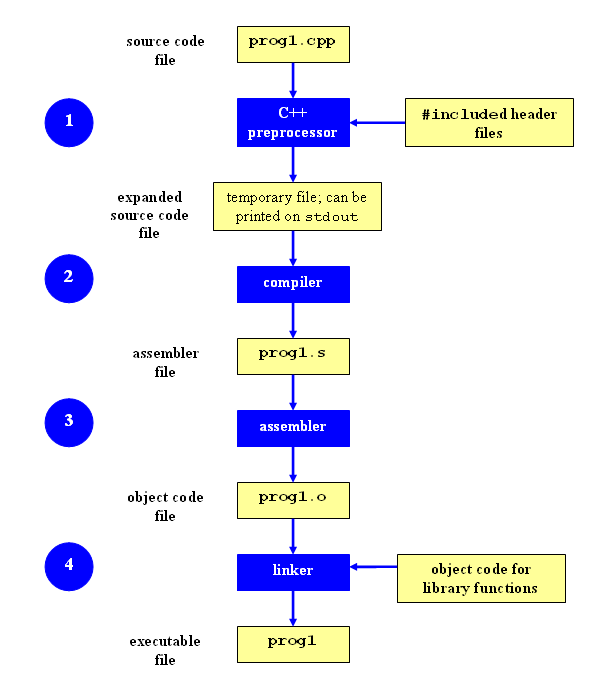
\includegraphics[width=6cm, height=6.5cm]{Term_3/Source/Pictures/compile.png}
\end{multicols}
\end{frame}

\subsection{Компиляция}
\begin{frame}[fragile]{Компиляция}
\begin{enumerate}
    \item Токенизация
    \item Построение промежуточного дерева по грамматике
    \item Построение abstract-syntax tree (AST)
    \item Построение платформо-зависимого дерева
    \item Создание ассемблерного кода.
\end{enumerate}
\end{frame}

\subsection{Линковка}
\begin{frame}[fragile]{Линковка}
На выходе с компилятора приходят объектные файлы. Они ничего не знают о существовании друг друга и их надо объединить в один, заполнив их "пропуски". Пример одиночного объектного файла:
 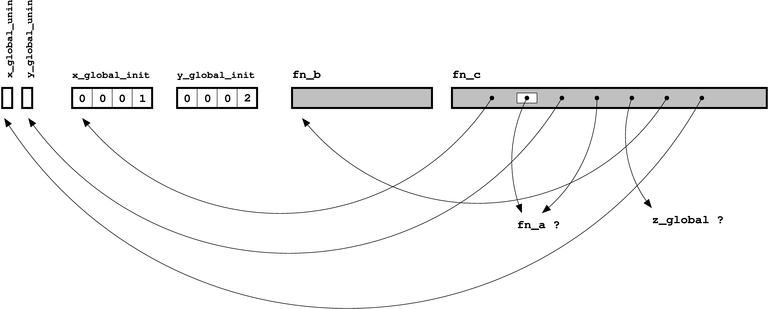
\includegraphics[width=12cm, height=5cm]{Term_3/Source/Pictures/c_parts.png}
\end{frame}

\begin{frame}[fragile]{Линковка - собранный файл}
Пример собранного исполняемого файла:
 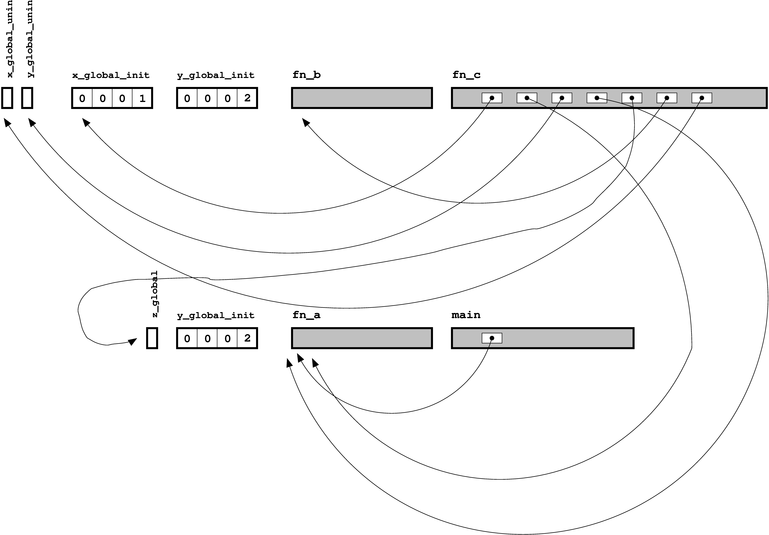
\includegraphics[width=10cm, height=7cm]{Term_3/Source/Pictures/c_parts_linked.png}
\end{frame}

\subsection{Загрузка исполняемого файла}
\begin{frame}{Загрузка исполняемого файла}
\begin{enumerate}
\item Глобальные переменные кладутся в память процесса as is.
\item Локальные переменные кладутся на стек, который растёт при вызовах функций и уменьшается при их завершении.
\item Динамические переменные расходуют память кучи, системные malloc и free управляют этой частью процесса.
\item bss - фрагмент неинициализированных пременных, заполнен нулями
\item Кроме того, на затронут mapping файлов в память и пространство ядра (kernel space).
\end{enumerate}
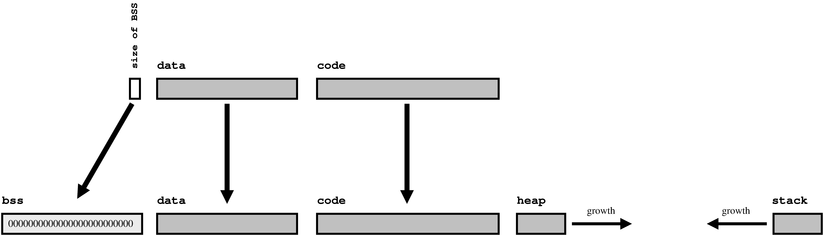
\includegraphics[width=11cm, height=3cm]{Term_3/Source/Pictures/os_map.png}
\end{frame}

\section{Библиотеки}
\subsection{Статические библиотеки}
\begin{frame}{Статические библиотеки}
\begin{enumerate}
\item Самая простая версия библиотек
\item Linux: lib*.a, Windows: *.lib
\item Библиотека может состоять из нескольких .o файлов.
\item Библиотека участвует в линковке объектными файлами, то есть тянется не вся библиотека, а только объектники, которые заполняют какой-либо 'пропуск'. При этом, тянется всё, что есть в этом объектном файле, в том числе новые 'пропуски'.
\item Линковка библиотек только после линковки частей программы, и только если есть 'пропуски'.
\item Библиотеки линкуются строго по порядку. Если вдруг библиотека-2 (идущая после библиотеки-1) требует что-то, что есть в незагруженном объектнике библиотеки-1, линкер это что-то не найдёт!

\end{enumerate}
\end{frame}

\subsection{Shared библиотеки}
\begin{frame}{Проблемы статических библиотек}
\begin{enumerate}
\item Каждый исполняемый файл содержит копию библиотеки $\rightarrow$ исполняемые файлы занимают кучу места.
\item Если мы хотим поменять код библиотеки нужно перелинковывать ВСЕ исполняемые файлы.
\end{enumerate}
\end{frame}

\subsection{Shared библиотеки}
\begin{frame}{Shared библиотеки}
\begin{enumerate}
\item *.so, *.dll, *.dylib.
\item Линкер просто оставляет некоторые 'пропуски' открытыми, записывая, что они должны заполняться из такой-то shared библиотеки.
\item Код библиотеки не включается в исполняемый файл.
\item Во время запуска программы (до исполнения main) операционная система натравливает маленькую версию линкера (ld.so) на оставшиеся 'пропуски'.
\item Если мы захотим поменять код, скажем, printf - нам не нужно перелинковывать все исполняемые файлы. 
\item Загрузка shared библиотек происходит целиком, а не по объектным файлам!
\item $ldd$ <имя исполняемого файла> чтобы посмотреть, какие библиотеки он захватывает.
\end{enumerate}
\end{frame}

\begin{frame}{Windows DLL}
\begin{enumerate}
\item{ Нужно явно указывать символы для экспорта одним из 3 вариантов:
    \begin{enumerate}
        \item \_\_declspec(dllexport) int my\_exported\_function(int x, double y);
        \item LINK.EXE /dll /export:my\_exported\_function
        \item LINK.EXE /dll /DEF:def\_file
    \end{enumerate}
}
\item Инормация об экспортируемых символах и их местонахождении хранится в .lib файле (не статическая библиотека, другое!). Этот файл нужен исполняемому, чтобы корректно слинковать DLL.
\item{ Можно ещё задавать импорты для лучшей оптимизации:
    \begin{enumerate}
        \item \_\_declspec(dllimport) int function\_from\_some\_dll(int x, double y);
        \item \_\_declspec(dllimport) extern int global\_var\_from\_some\_dll;
    \end{enumerate}
}
\end{enumerate}
\end{frame}

\begin{frame}{Windows DLL}
Что может получиться после линковки:
    \begin{enumerate}
        \item library.DLL: код и данные библиотеки, непосредственно используется исполняемым файлом.
        \item library.LIB: файл, в котором описываются экспортируемые DLL символы.
        \item library.EXP: ещё один файл с описаниями симоловов, нужен для разрешения циклических зависимостей.
        \item library.ILK: при опции линкера /INCREMENTAL, хранит состояние инкрементальной компоновки, для ускорения перекомпиляции.
        \item library.PDB: при опции линкера /DEBUG, содержит отладочные данные и сведения о состоянии проекта, например информацию о типах.
        \item library.MAP: при опции линкера /MAP, хранит расположение функций и данных в DLL.
    \end{enumerate}
\end{frame}
\begin{frame}{Windows DLL}
Что может быть до линковки:
    \begin{enumerate}
        \item library.LIB: файлы других библиотек, в которых описываются экспортируемые ими символы.
        \item library.LIB: статические библиотеки - набор объектных файлов. Неоднозначное расширение :)
        \item library.DEF: определение библиотеки, контроль некоторых настроек библиотеки, в частности - в нём можно задавать экспортируемые символы.
        \item library.EXP: файл с описаниями симоловов линкуемых библиотек, нужен для разрешения циклических зависимостей.
        \item library.ILK: см. выше.
        \item library.RES: ресурсный файл с разными GUI штуками, локализациями и всем таким, это всё нужно исполняемому файлу
    \end{enumerate}
\end{frame}

\subsection{Динамически загружаемые библиотеки}
\begin{frame}{Динамически загружаемые библиотеки (настоящие DLL)}
\begin{enumerate}
\item Загрузка бибилиотеки в любом месте программы, не только до main.
\item dlopen и dlsym (или LoadLibrary и GetProcAddress).
\item dlopen - берёт библиотеку и загружает её в память процесса.
\item dlsym - берёт имя символа и возвращает указатель на его местонахождение в в загруженной области памяти.
\end{enumerate}
\end{frame}

\section{C++ - mangling}
\subsection{Перегрузка функций}
\begin{frame}{Перегрузка функций}
\begin{enumerate}
\item В Си нельзя перегружать функции, в C++ можно.
\item Пример: int max(int x, int y); float max(float x, float y);
\item А что делать линкеру, он же по имени символы ищет?
\end{enumerate}
\end{frame}

\begin{frame}{Mangling}
\begin{enumerate}
\item Решение: {
\begin{enumerate}
    \item int max(int x, int y) -> имя - \_Z3maxii
    \item float max(float x, float y) -> имя - \_Z3maxff
\end{enumerate}
}
\item Всё сложнее для классов.
\item И ещё сложнее для шаблонов.
\item extern \quotes{C} у объявления и определения - убирает mangling для совместимости кода на Си и C++.
\item extern \quotes{C} игнорируется методами класса.
\end{enumerate}
\end{frame}

\subsection{Конструкторы статических объектов}
\begin{frame}{Конструкторы статических объектов}
\begin{enumerate}
\item В Си инициализация статических объектов очень простая - просто копируем данные из data секции в память.
\item В C++ появились конструкторы.
\item Компилятор обязан составить список конструкторов, которые нужно вызвать перед запуском программы и включить в программу код, который все эти конструкторы вызовет.
\item В рамках одной единицы трансляции порядок конструирования закреплён.
\item Но в каком порядке конструкторы будут вызываться из разных единиц трансляции - неизвестно, будьте осторожны, особенно если они друг от друга зависят!
\end{enumerate}
\end{frame}

\appendix
\section<presentation>*{\appendixname}
\subsection<presentation>*{Useful links}

\begin{frame}[allowframebreaks]
  \frametitle<presentation>{Полезные ссылки}
    
  \begin{thebibliography}{10}
{
  \beamertemplatebookbibitems
  % Start with overview books.
    
\bibitem{standard}
  \texttt{C++11 n3690}
  \newblock \href{http://www.open-std.org/jtc1/sc22/wg21/docs/papers/2013/n3690.pdf}{\texttt{http://www.open-std.org/jtc1/sc22/wg21/docs/\\papers/2013/n3690.pdf}}

  \bibitem{link01}
  \texttt{Статья про линковку}
  \newblock \href{https://www.lurklurk.org/linkers/linkers.html#cfile}{\texttt{https://www.lurklurk.org/linkers/linkers.html#cfile}}
  
  \bibitem{odr01}
  \texttt{Habr: ODR}
  \newblock \href{https://habrahabr.ru/company/abbyy/blog/108166/}{\texttt{https://habrahabr.ru/company/abbyy/blog/108166/}}
  
  \bibitem{odr02}
  \texttt{SO: ODR}
   \newblock \href{https://ru.stackoverflow.com/questions/418755/\%D0\%A7\%D1\%82\%D0\%BE-\%D1\%82\%D0\%B0\%D0\%BA\%D0\%BE\%D0\%B5-\%D0\%9F\%D1\%80\%D0\%B0\%D0\%B2\%D0\%B8\%D0\%BB\%D0\%BE-\%D0\%BE\%D0\%B4\%D0\%BD\%D0\%BE\%D0\%B3\%D0\%BE-\%D0\%BE\%D0\%BF\%D1\%80\%D0\%B5\%D0\%B4\%D0\%B5\%D0\%BB\%D0\%B5\%D0\%BD\%D0\%B8\%D1\%8F-one-definition-rule}{\texttt{https://ru.stackoverflow.com/questions/418755/\\Что-такое-Правило-одного-определения-one-definition-rule}}
    
    \bibitem{compilation-schema}
  \texttt{The C++ compilation process}
   \newblock \href{http://faculty.cs.niu.edu/~mcmahon/CS241/Notes/compile.html}{\texttt{ http://faculty.cs.niu.edu/~mcmahon/CS241/Notes/compile.html}}
   
    \bibitem{memory}
  \texttt{Хабр: Организация памяти}
   \newblock \href{https://habrahabr.ru/company/smart_soft/blog/185226/}{\texttt{https://habrahabr.ru/company/smart_soft/blog/185226/}}
   
  
}
    
  \end{thebibliography}
\end{frame}

\end{document}


